\documentclass[tikz, border=3mm]{standalone}
\usetikzlibrary{arrows.meta, positioning, shapes}

\begin{document}
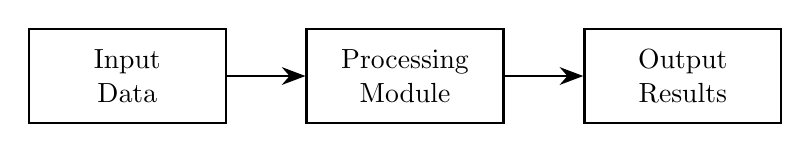
\begin{tikzpicture}[
    % Define node styles
    box/.style={rectangle, draw=black, thick, minimum width=2.5cm,
                minimum height=1.2cm, align=center, fill=white}
]
    % Create nodes
    \node[box] (input) {Input\\Data};
    \node[box, right=of input] (process) {Processing\\Module};
    \node[box, right=of process] (output) {Output\\Results};

    % Draw arrows between nodes
    \draw[-{Stealth[length=3mm]}, thick] (input) -- (process);
    \draw[-{Stealth[length=3mm]}, thick] (process) -- (output);
\end{tikzpicture}
\end{document}
